\subsection{Klassediagram}
For at illustrere modellaget i vores MVC-mønster, har vi produceret et klassediagram (se \myref{diagram:klassediagram}) i UML, der simplificerer strukturen. 
Dette diagram er en implementering af vores struktur fra problemområdeanalysen på \myref{figur:PDklasse}.

\begin{figure}[h]
\centering
 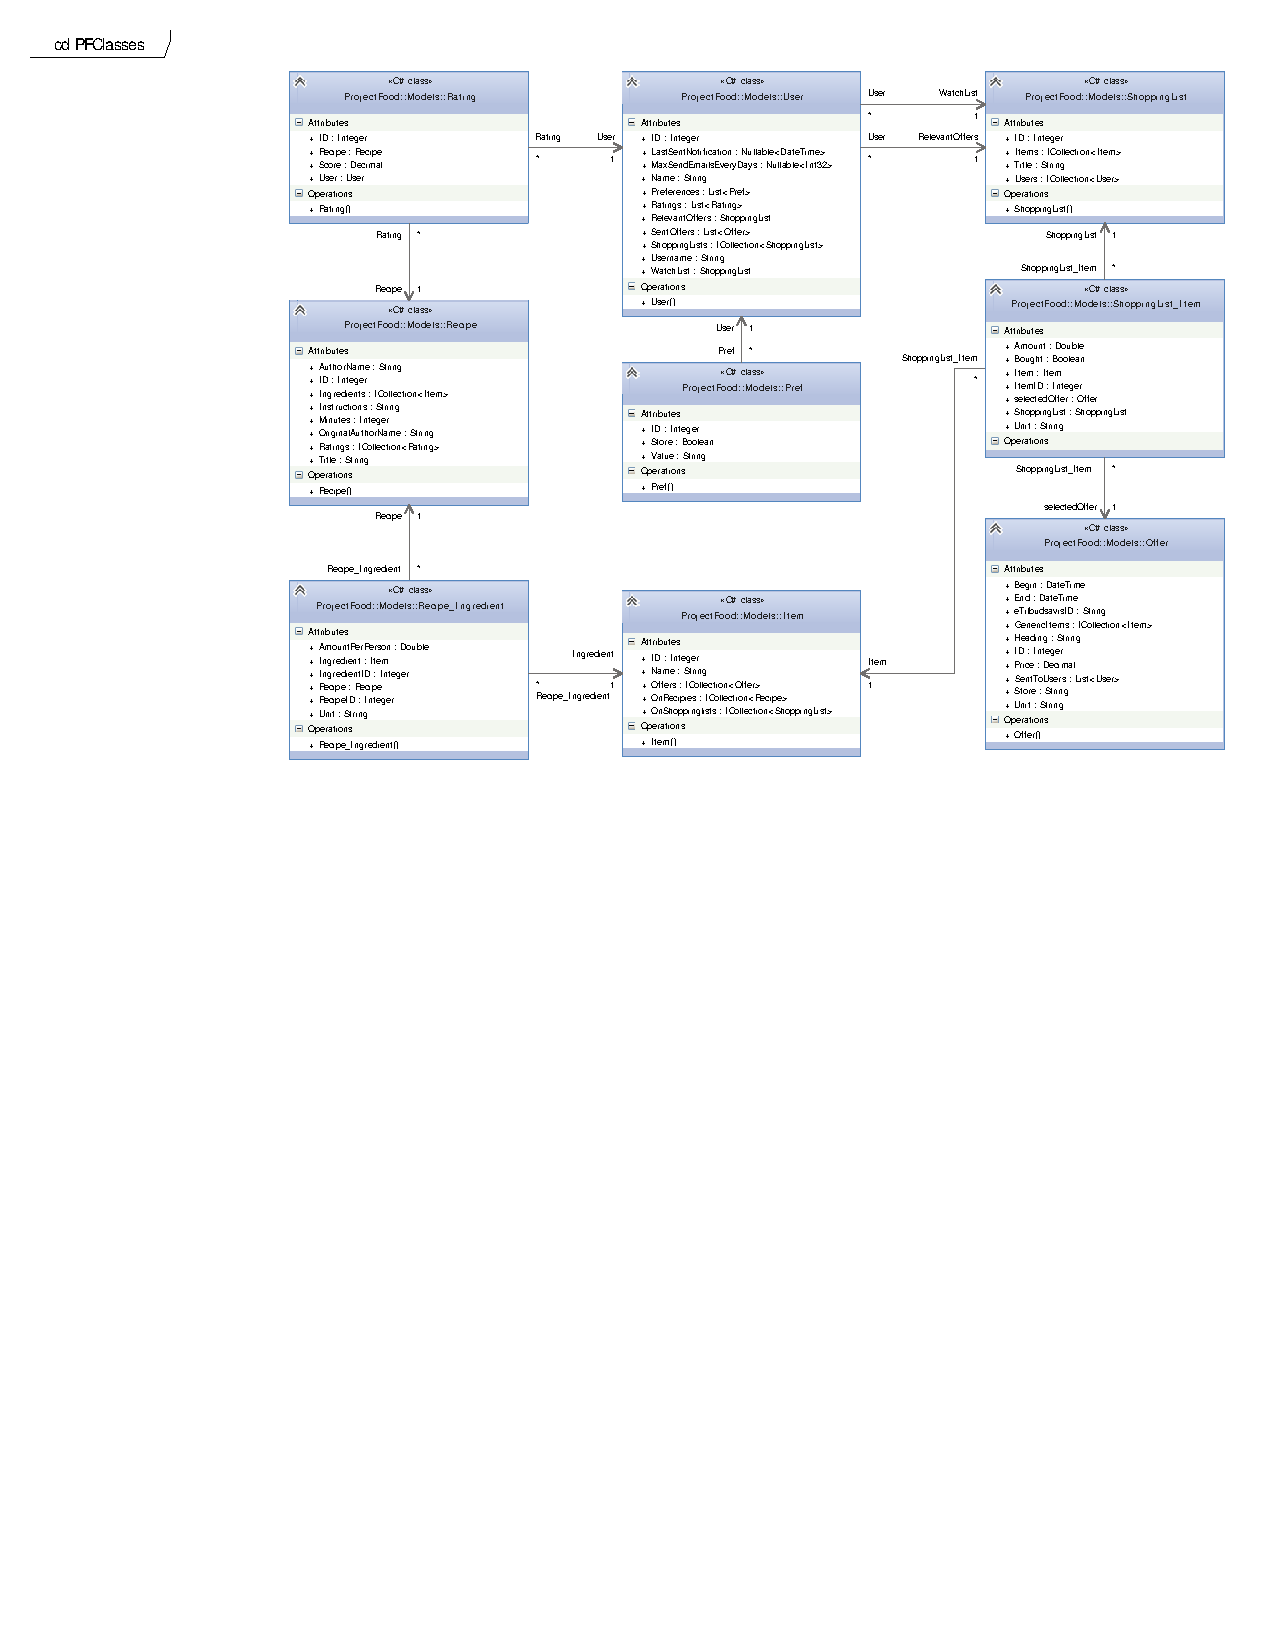
\includegraphics[trim=4.85cm 15cm 0.85cm 1cm, clip, width=1\textwidth]{/Diagrams/PFClasses.pdf}
\caption{UML klassediagram for modellaget i MVC-mønsteret}\label{diagram:klassediagram}
\end{figure}

Der er mange relationer mellem klasserne, da de forskellige klasser indeholder lister af hinanden.
En \class{ShoppingList} har en liste over \class{Items}, og disse \class{Items} har en liste over \class{Offers}, for at binde Offers til det pågældende Item.
\class{Recipe} har en liste over \class{Items}, som bruges som ingredienser.
På denne måde kan de tilføjes til \class{ShoppingList} gennem \class{RecipesController}, uden at skulle lave nye objekter, som \class{ShoppingList} kan læse.
\class{User} har en liste over \class{ShoppingLists}, samt en liste over \class{Prefs}, eller præferencer som angiver hvilke tilbud der skal filtreres væk, for at gøre hjemmesiden mere personlig og fokuseret på brugeren som er logget ind.
Der er relationstabeller for many-to-many forholdene, som yderligere gør det muligt at gemme værdier ved hvert forhold, eksempelvis mængder (\class{Amount}) på en \class{ShoppingList}.
Dette gøres igennem relationsklasserne, \class{Recipe\textunderscore Ingredient}, og \class{ShoppingList\textunderscore item}.
I \myref{sec:struktur} blev anbefaling oprettet som en klasse, i vores implementering fungerer anbefaling som en sortering af viste opskrifter, læs mere om dette i \myref{anbefaling} om anbefaling.

I de følgende afsnit, vil der gives en gennemgang af udvalgte dele af komponenterne fra \myref{subsec:komp}.
